\begin{figure}[H]
    \centering
    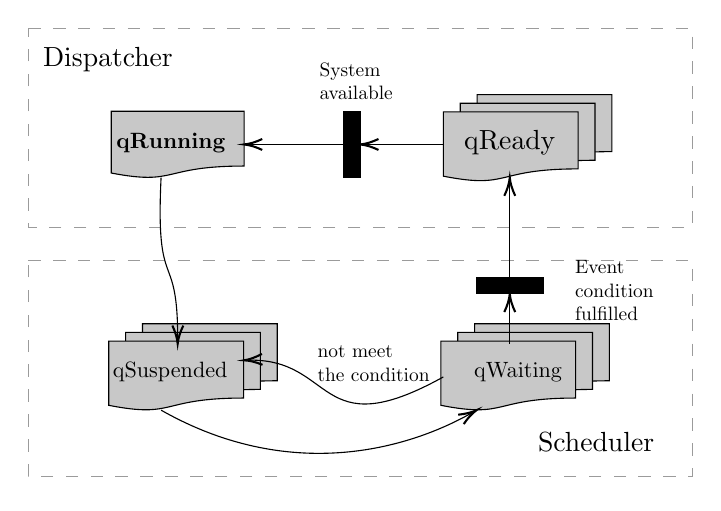
\begin{tikzpicture}[x=0.75pt,y=0.75pt,yscale=-1,xscale=1,scale=0.8]
        \draw  [fill={rgb, 255:red, 200; green, 200; blue, 200 }  ,fill opacity=1 ] (378.8,188) -- (460,188) -- (460,222.32) .. controls (409.25,222.32) and (419.4,234.7) .. (378.8,226.69) -- cycle ; \draw  [fill={rgb, 255:red, 200; green, 200; blue, 200 }  ,fill opacity=1 ] (368.65,193.2) -- (449.85,193.2) -- (449.85,227.52) .. controls (399.1,227.52) and (409.25,239.9) .. (368.65,231.89) -- cycle ; \draw  [fill={rgb, 255:red, 200; green, 200; blue, 200 }  ,fill opacity=1 ] (358.5,198.4) -- (439.7,198.4) -- (439.7,232.72) .. controls (388.95,232.72) and (399.1,245.1) .. (358.5,237.09) -- cycle ;
        \draw  [fill={rgb, 255:red, 200; green, 200; blue, 200 }  ,fill opacity=1 ] (178.8,188) -- (260,188) -- (260,222.32) .. controls (209.25,222.32) and (219.4,234.7) .. (178.8,226.69) -- cycle ; \draw  [fill={rgb, 255:red, 200; green, 200; blue, 200 }  ,fill opacity=1 ] (168.65,193.2) -- (249.85,193.2) -- (249.85,227.52) .. controls (199.1,227.52) and (209.25,239.9) .. (168.65,231.89) -- cycle ; \draw  [fill={rgb, 255:red, 200; green, 200; blue, 200 }  ,fill opacity=1 ] (158.5,198.4) -- (239.7,198.4) -- (239.7,232.72) .. controls (188.95,232.72) and (199.1,245.1) .. (158.5,237.09) -- cycle ;
        \draw  [fill={rgb, 255:red, 200; green, 200; blue, 200 }  ,fill opacity=1 ] (380.3,50) -- (461.5,50) -- (461.5,84.32) .. controls (410.75,84.32) and (420.9,96.7) .. (380.3,88.69) -- cycle ; \draw  [fill={rgb, 255:red, 200; green, 200; blue, 200 }  ,fill opacity=1 ] (370.15,55.2) -- (451.35,55.2) -- (451.35,89.52) .. controls (400.6,89.52) and (410.75,101.9) .. (370.15,93.89) -- cycle ; \draw  [fill={rgb, 255:red, 200; green, 200; blue, 200 }  ,fill opacity=1 ] (360,60.4) -- (441.2,60.4) -- (441.2,94.72) .. controls (390.45,94.72) and (400.6,107.1) .. (360,99.09) -- cycle ;
        \draw  [color={rgb, 255:red, 155; green, 155; blue, 155 }  ,draw opacity=1 ][dash pattern={on 4.5pt off 4.5pt}] (110,10) -- (510,10) -- (510,130) -- (110,130) -- cycle ;
        \draw  [fill={rgb, 255:red, 200; green, 200; blue, 200 }  ,fill opacity=1 ] (160,60) -- (240,60) -- (240,93) .. controls (190,93) and (200,104.9) .. (160,97.2) -- cycle ;
        \draw  [color={rgb, 255:red, 155; green, 155; blue, 155 }  ,draw opacity=1 ][dash pattern={on 4.5pt off 4.5pt}] (110,150) -- (510,150) -- (510,280) -- (110,280) -- cycle ;
        \draw    (360,220) .. controls (283.27,262.57) and (295.25,208.11) .. (241.64,209.93) ;
        \draw [shift={(240,210)}, rotate = 356.90999999999997] [color={rgb, 255:red, 0; green, 0; blue, 0 }  ][line width=0.75]    (10.93,-3.29) .. controls (6.95,-1.4) and (3.31,-0.3) .. (0,0) .. controls (3.31,0.3) and (6.95,1.4) .. (10.93,3.29);
        \draw    (190,240) .. controls (266.73,283.56) and (338.06,264.39) .. (378.78,240.72) ;
        \draw [shift={(380,240)}, rotate = 509.35] [color={rgb, 255:red, 0; green, 0; blue, 0 }  ][line width=0.75]    (10.93,-3.29) .. controls (6.95,-1.4) and (3.31,-0.3) .. (0,0) .. controls (3.31,0.3) and (6.95,1.4) .. (10.93,3.29)   ;
        \draw  [fill={rgb, 255:red, 0; green, 0; blue, 0 }  ,fill opacity=1 ] (420,160) -- (380,160) -- (380,170) -- (420,170) -- cycle ;
        \draw  [fill={rgb, 255:red, 0; green, 0; blue, 0 }  ,fill opacity=1 ] (310,60) -- (300,60) -- (300,100) -- (310,100) -- cycle ;
        \draw    (400,200) -- (400,172) ;
        \draw [shift={(400,170)}, rotate = 450] [color={rgb, 255:red, 0; green, 0; blue, 0 }  ][line width=0.75]    (10.93,-3.29) .. controls (6.95,-1.4) and (3.31,-0.3) .. (0,0) .. controls (3.31,0.3) and (6.95,1.4) .. (10.93,3.29)   ;
        \draw    (400,160) -- (400,102) ;
        \draw [shift={(400,100)}, rotate = 450] [color={rgb, 255:red, 0; green, 0; blue, 0 }  ][line width=0.75]    (10.93,-3.29) .. controls (6.95,-1.4) and (3.31,-0.3) .. (0,0) .. controls (3.31,0.3) and (6.95,1.4) .. (10.93,3.29)   ;
        \draw    (360,80) -- (312,80) ;
        \draw [shift={(310,80)}, rotate = 360] [color={rgb, 255:red, 0; green, 0; blue, 0 }  ][line width=0.75]    (10.93,-3.29) .. controls (6.95,-1.4) and (3.31,-0.3) .. (0,0) .. controls (3.31,0.3) and (6.95,1.4) .. (10.93,3.29)   ;
        \draw    (300,80) -- (242,80) ;
        \draw [shift={(240,80)}, rotate = 360] [color={rgb, 255:red, 0; green, 0; blue, 0 }  ][line width=0.75]    (10.93,-3.29) .. controls (6.95,-1.4) and (3.31,-0.3) .. (0,0) .. controls (3.31,0.3) and (6.95,1.4) .. (10.93,3.29)   ;
        \draw    (190,100) .. controls (186.54,172.27) and (200.22,140.65) .. (200.01,198.23) ;
        \draw [shift={(200,200)}, rotate = 270.48] [color={rgb, 255:red, 0; green, 0; blue, 0 }  ][line width=0.75]    (10.93,-3.29) .. controls (6.95,-1.4) and (3.31,-0.3) .. (0,0) .. controls (3.31,0.3) and (6.95,1.4) .. (10.93,3.29)   ;
        \draw (196,79) node  [scale=0.8, align=left] {\textbf{qRunning}};
        \draw (195.5,217) node [scale=0.8] [align=left] {qSuspended};
        \draw (405,217) node [scale=0.8] [align=left] {qWaiting};
        \draw (400,79) node [scale=1] [align=left] {qReady};
        \draw (158,29) node  [align=left] {Dispatcher};
        \draw (452,259) node  [align=left] {Scheduler};
        \draw (307.5,42) node [scale=0.7] [align=left] {System \\available};
        \draw (318,212) node [scale=0.7] [align=left] {not meet\\the condition};
        \draw (463,168) node [scale=0.7] [align=left] {Event\\condition\\fulfilled};
    \end{tikzpicture}
    \caption{Task global states}
    \label{fig:scheduler_states}
\end{figure}